\subsection{Graphical Method}
\label{subsection:spreadmethod}
\subsubsection{Atlantic Ocean}
\label{subsubsection:spreadmethodatlanticocean}

One of the aims of this work was to reproduce the diagrams given in \citet{McDougall1987} to illustrate the spread of $\theta$ and $S$ on various surfaces of interest.  In reference to figure \ref{fig:theory_mcdougall_theta_spread} (also given in Appendix \ref{appendix_a} as figure \ref{fig:appendix_mcdougall_theta_spread}) the first surfaces of interest were decided upon. These were $\sigma_0 = 27.73$, $\sigma_2 = 36.84$ and the neutral surface known in the paper as ``Nsa". The paper also includes $\sigma_0 = 27.83$ but it was decided not to included this surface as it was similar to the other $\sigma_0$ surface. The $\sigma_0 = 27.73$ was considered more important as it was closer to $\sigma_0 = 27.75$, which had been used to calculate the $\gamma_n$ surface. In addition, it was decided to include the $\sigma_4$ surface in order to better understand the trend of the spread of $\theta$ and $S$.

In the original McDougall (1987) paper the neutral surface, which we will refer to  as  a $\gamma_n$ surface,  was  calculated  for  this  specific  case.  However,  in  the  WOCE dataset the values of $\gamma_n$ have already been supplied.  Therefore in order to match the value given in the paper linear interpolation was used in order to project $\gamma_n$ on to the $\sigma_0= 27.75$ surface at 5◦N and 47◦W.  This produced a value of $\gamma_n= 27.89$.

In order to find a $\sigma_4$ surface a similar process was undertaken, but interpolating $\sigma_4$ data onto the $\gamma_n = 27.89$ surface. This resulted in a value of $\sigma_4 = 45.51$. The list of surfaces to be considered was:

\begin{itemize}
    \item $\sigma_0= 27.73$ 
    \item $\sigma_2= 36.84$ 
    \item $\sigma_4= 45.51$ 
    \item Neutral surface``Nsa" referred to from now on as $\gamma_n= 27.75$
\end{itemize}

In order to project $S$ and $\theta$ onto the density surfaces two methods were originally considered: a polynomial spline method and linear interpolation. The former involves fitting polynomials piece-wise to the data in order to create a vertical profile. The latter takes the two points of interest and treats the profile between them as linear. The spline method is usually more accurate as it gives a closer fit to the likely vertical profile than linear interpolation but is more expensive computationally.  When we compared the two methods, as seen in figure \ref{fig:polyvslinear}, there
was little difference in the results. Therefore linear interpolation was chosen as it
is significantly cheaper computationally but has a similar level of accuracy as the spline method.

\begin{figure}[htbp]
    \centering
    \begin{subfigure}[b]{0.4\textwidth}
         \centering
         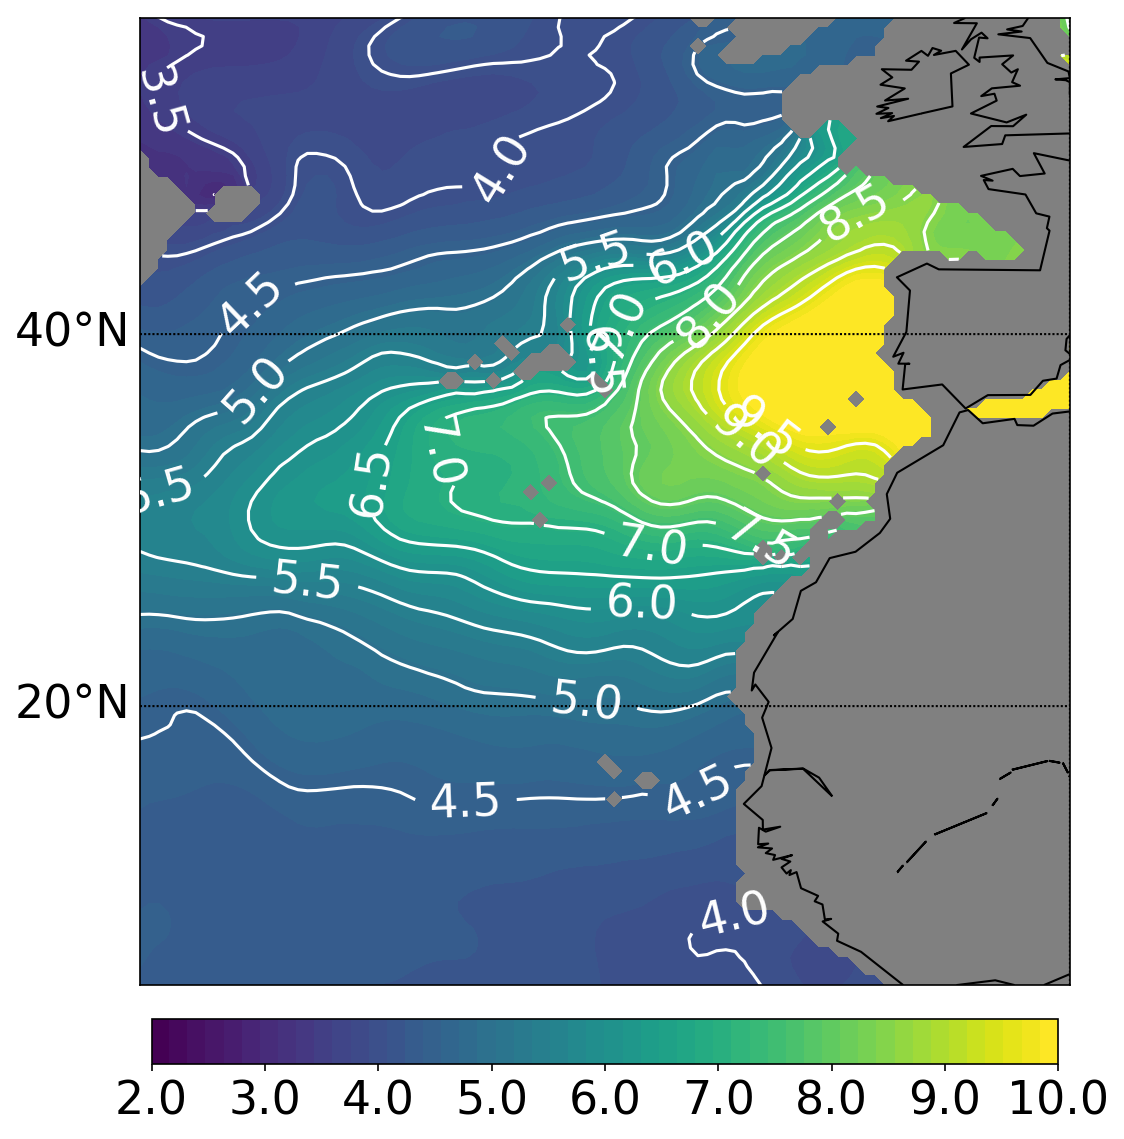
\includegraphics[width=\textwidth]{spline_method_example}
         \caption{Spline method}
         \label{fig:subplot_poly_spline}
     \end{subfigure}
     \hfill
     \begin{subfigure}[b]{0.4\textwidth}
         \centering
         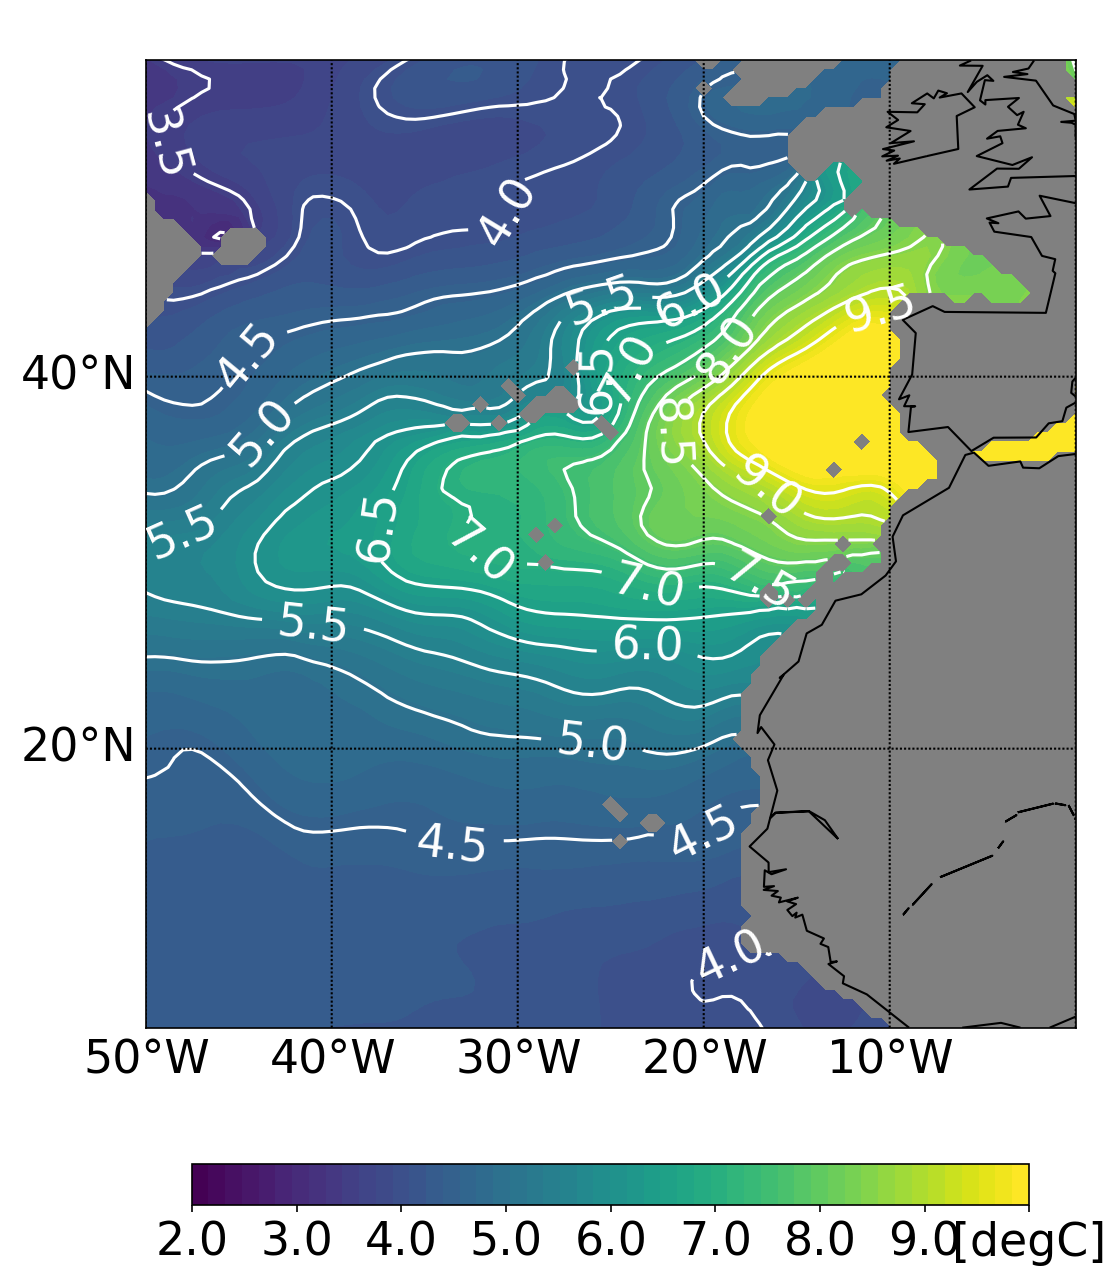
\includegraphics[width=\textwidth]{linear_method_example}
         \caption{Linear interpolation}
         \label{fig:subplot_linear_inter}
     \end{subfigure}
    \caption{$\theta$ projected onto the surface $\sigma_0 = 27.73$ using two different interpolation methods}
    \label{fig:polyvslinear}
\end{figure}

\subsubsection{Gibraltar Straight}
\label{subsubsection:spreadmethodgibraltarstraight}

In order to better understand the alignment of the preferred mixing direction and the density surfaces the Gibraltar Straight was considered. It was decided that following the outflow of high salinity water from the Mediterranean closer to the source would be a more appropriate test than the original location at 5$^{\circ}$N and 47$^{\circ}$W. The new location was chosen at 36$^{\circ}$N and 8$^{\circ}$W. While the Straight itself is closer to 
6$^{\circ}$W, this location was chosen as the dataset contained data-points to a depth of over 1500m. 

The vertical profile of salinity was then considered at this point and the depth of the salinity maximum was found. At this location there was a maximum near the surface and another at 1200m depth. The latter was chosen because this is closest to the expected depth of the Mediterranean salinity tongue in this area. This can be seen in figure \ref{fig:salinitycrosssectionWOCE} which was given in section \ref{section:lit_review_mixing}. 

The values of $\gamma_n$, $\sigma_0$, $\sigma_2$ and $\sigma_4$ were then found at this depth and location. These were as follows (given to 4 d.p.):

\begin{itemize}
    \item $\sigma_0= 27.7974$
    \item $\sigma_2= 36.5717$
    \item $\sigma_4= 44.9612$
    \item $\gamma_n= 27.7736$
\end{itemize}

As for the Atlantic ocean interior in section \ref{subsubsection:spreadmethodatlanticocean}, linear interpolation was used to project $S$ and $\theta$ onto the density surfaces of interest. 

